\documentclass[12pt]{article}

%%%%%%%%%%%%%%%%%%%%%%%%%%%%%%%%%%%%%%%%%%%%%%%%%%%%%%%%%%%%%%%%%%%%%%%%%%
\usepackage{amsmath}
\usepackage{bbm}
\usepackage{amssymb}
\usepackage{enumerate}
\usepackage{dcolumn}
\usepackage{graphicx}
\usepackage{makeidx}
\usepackage{amsfonts}
\usepackage[bottom]{footmisc}
\usepackage{booktabs}
%\usepackage{enumitem}
\usepackage{eurosym}
\usepackage[latin1]{inputenc}
\usepackage{lscape}
\usepackage{color}
\usepackage{setspace}
\usepackage[longnamesfirst]{natbib}
\usepackage[flushleft]{threeparttable}
\bibpunct{\color{black}{(}}{\color{black}{)}}{;}{a}{}{,}
%  \bibpunct{(}{)}{;}{a}{}{,}
%  \bibpunct{[}{]}{;}{a}{}{,}
%\usepackage[metapost]{mfpic}
%  \opengraphsfile{pics}
\usepackage{ifthen}
\usepackage[colorlinks]{hyperref}
\hypersetup{  colorlinks = {true},
	%allcolors={black},
	urlcolor={black},
	citecolor={blue},
	linkcolor={black},
	anchorcolor={black}
	filecolor={black}
}
\usepackage{xcolor}
\usepackage{soul,color}
\soulregister\cite7
\soulregister\citealt7
\soulregister\citeauthor7
\soulregister\citeyear7
\soulregister\ref7
\soulregister\eqref7
\soulregister\pageref7
\renewcommand{\theequation}{\thesection.\arabic{equation}}

% OVER-FULL BOX CONTROLS -------------------------------------------------
%%%%%%%%%%%%%%%%%%%%%%%%%%%%%%%%%%%%%%%%%%%%%%%%%%%%%%%%%%%%%%%%%%%%%%%%%%
% Over-full v-boxes on even pages are due to the \v{c} in author's name
\vfuzz2pt % Don't report over-full v-boxes if over-edge is small
\hfuzz2pt % Don't report over-full h-boxes if over-edge is small




% PAGE DEFINITION --------------------------------------------------------
%%%%%%%%%%%%%%%%%%%%%%%%%%%%%%%%%%%%%%%%%%%%%%%%%%%%%%%%%%%%%%%%%%%%%%%%%%
\usepackage[textheight=9in,textwidth=6.5in]{geometry}
\parindent=0.23in
\parskip=1pt


\usepackage{epstopdf}
\usepackage{setspace}
\usepackage{titlesec}
\titleformat{\section}
{\normalfont\Large\bfseries}
{Appendix \thesection.}{0.5em}{}
\titleformat{\subsection}
{\normalfont\large\bfseries}
{\thesubsection.}{0.5em}{}
\titleformat{\subsubsection}
{\normalfont\normalsize\bfseries}
{\thesubsubsection.}{0.5em}{}
\bibpunct{\color{black}{(}}{\color{black}{)}}{;}{a}{}{,}
\usepackage{pdflscape}
\usepackage{comment}
\usepackage{relsize}
\newcommand{\blob}{\rule[.2ex]{1ex}{1ex}}
\setlength{\unitlength}{0.25cm}
\usepackage{lineno}
\usepackage{chngcntr}
\expandafter\def\expandafter\normalsize\expandafter{%
	\normalsize
	% \setlength\abovedisplayskip{10pt}
	\setlength\belowdisplayskip{16pt}
	% \setlength\abovedisplayshortskip{10pt}
	\setlength\belowdisplayshortskip{16pt}
}

\baselineskip=12pt


\renewcommand{\figurename}{\bf Figure RP}
\renewcommand{\tablename}{\bf Table RP}
\begin{document}
	

\clearpage
\newpage
\begin{figure}[h]
	\begin{centering}
		
		
		\textbf{Panel A: Deposit Spread} \\
		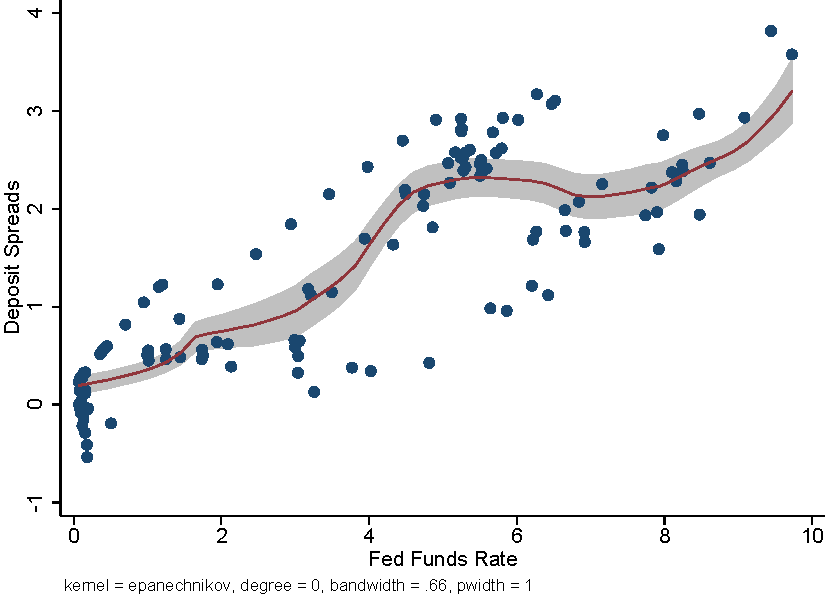
\includegraphics[scale=.8]{../output/Figures/lpoly_deposit_spread}
		
		\textbf{Panel B: Loan Spread} \\
		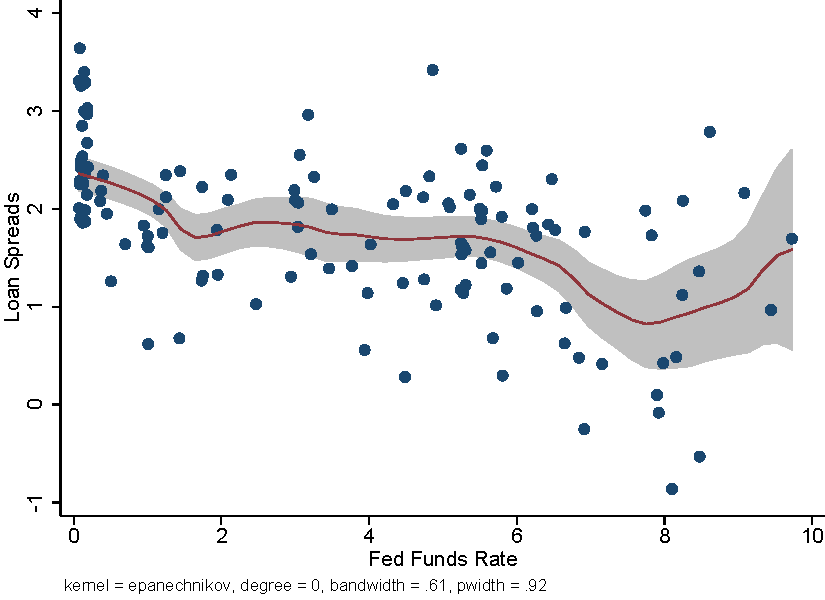
\includegraphics[scale=.8]{../output/Figures/lpoly_loan_spread}
		
		\par
		\caption{Deposit Spread, Loan Spread, and the Federal Funds Rate\label{fig:lpoly_deposit_spread}}
	\end{centering}
	{\footnotesize{In this figure, we plot kernel regressions of average deposit and loan spreads for U.S. banks on the federal funds rate.  We use an Epanechnikov kernel with a bandwidth of 0.66 for deposits and 0.61 for loans. The sample period is 1985--2017. The data frequency is quarterly.  The deposit and loan rates are constructed using the Call Reports, and the federal funds rate is  from the FRED database.}}
\end{figure}










\newpage
\begin{figure}[h]
	\begin{centering}
		High Federal Funds Rate
		\par\end{centering}
	\begin{centering}
		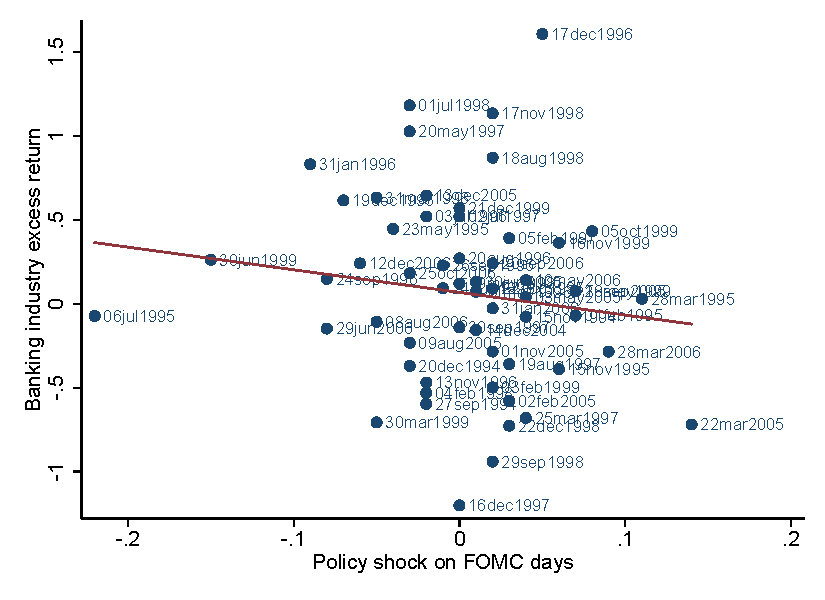
\includegraphics[scale=0.8]{../output/Figures/bank_treasury2y_above}
		\par\end{centering}
	\vspace{5mm}
	\begin{centering}
		Low Federal Funds Rate
		\par
		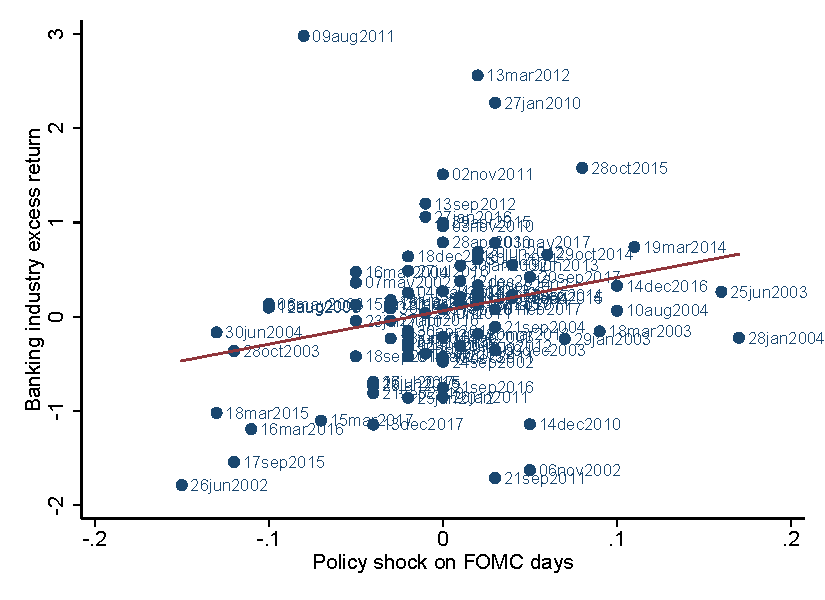
\includegraphics[scale=0.8]{../output/Figures/bank_treasury2y_below}
		\caption{Monetary Policy Shocks and Bank Equity Returns\label{fig:stock_return}}
	\end{centering}
	{\footnotesize{This figure provides scatter plots of bank industry excess returns against monetary policy shocks on FOMC days from 1994 to 2017. The excess  returns are defined as the difference between bank industry index returns and market returns. Monetary policy shocks are measured by one-day changes in two-year Treasury yields on FOMC days.
			The sample for the upper panel constitutes observations in which the starting level of the federal funds rate is above 2\%. The sample the lower panel constitutes observations in which the starting level of the federal funds rate is below 2\%.  We exclude observations during the collapse of the dot-com bubble (2000-2001) and the financial crisis (2007-2009).   Bank industry stock returns are  from Kenneth French's website, and the two-year Treasury yield is  from the FRED database.}}
\end{figure}



\newpage
\begin{figure}[h]
	\begin{centering}
		High Federal Funds Rate
		\par\end{centering}
	\begin{centering}
		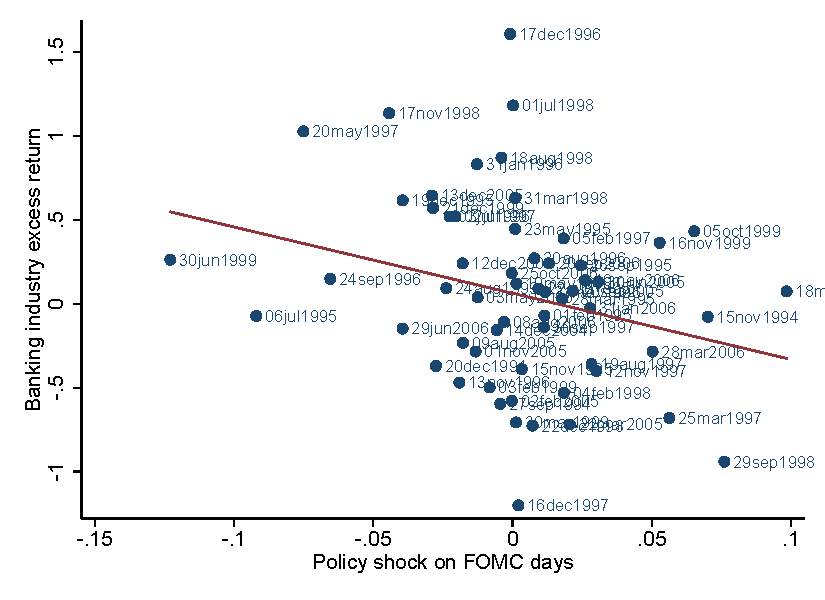
\includegraphics[scale=0.8]{../output/Figures/bank_karadi_above}
		\par\end{centering}
	\vspace{5mm}
	\begin{centering}
		Low Federal Funds Rate
		\par
		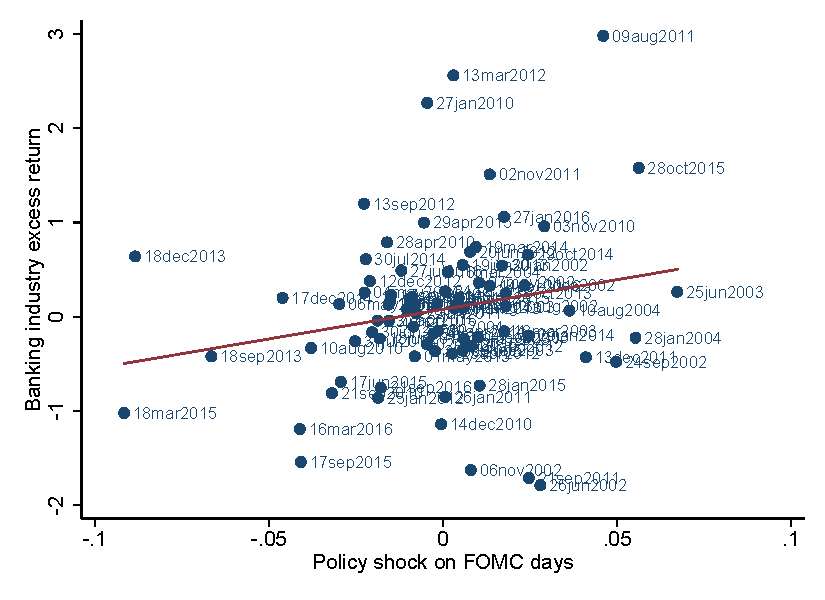
\includegraphics[scale=0.8]{../output/Figures/bank_karadi_below}
		\caption{Monetary Policy Shocks and Bank Equity Returns\label{fig:stock_return}}
	\end{centering}
	{\footnotesize{This figure provides the scatter plot of bank industry excess returns against monetary policy shocks on FOMC days from 1994 to 2017. The excess  returns are defined as the difference between bank industry index returns and the market returns. Monetary policy shocks are measured by the change in the 3-month federal funds future subtracting  central bank information shocks \citep{JarocinskiKaradi2018}. The sample for the upper panel constitutes observations in which the starting level of the federal funds rate is above 2\%. The sample for the lower panel constitutes observations in which the starting level of the federal funds rate is below 2\%. We exclude observations during the collapse of the dot-com bubble (2000-2001) and the financial crisis (2007-2009). Bank industry stock returns are  from Kenneth French's website and the monetary policy shocks are  from the website of the \textit{American Economic Journal: Macroeconomics}.}}
\end{figure}



\newpage
\begin{figure}[h]
	\begin{centering}
		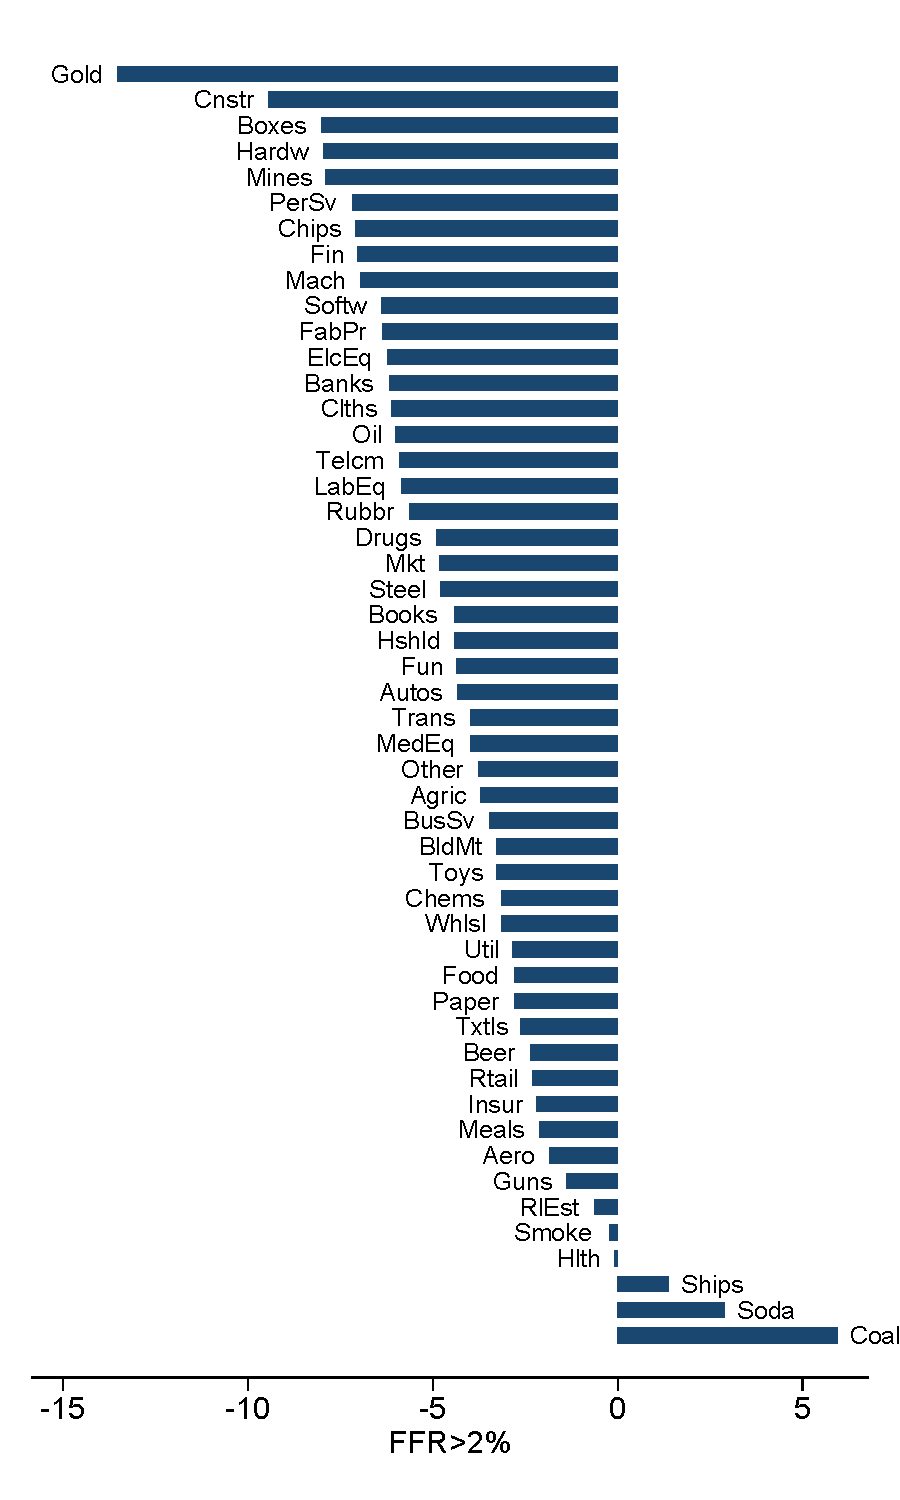
\includegraphics[scale=0.5]{../output/Figures/industry_fomc_bar_gt2}
		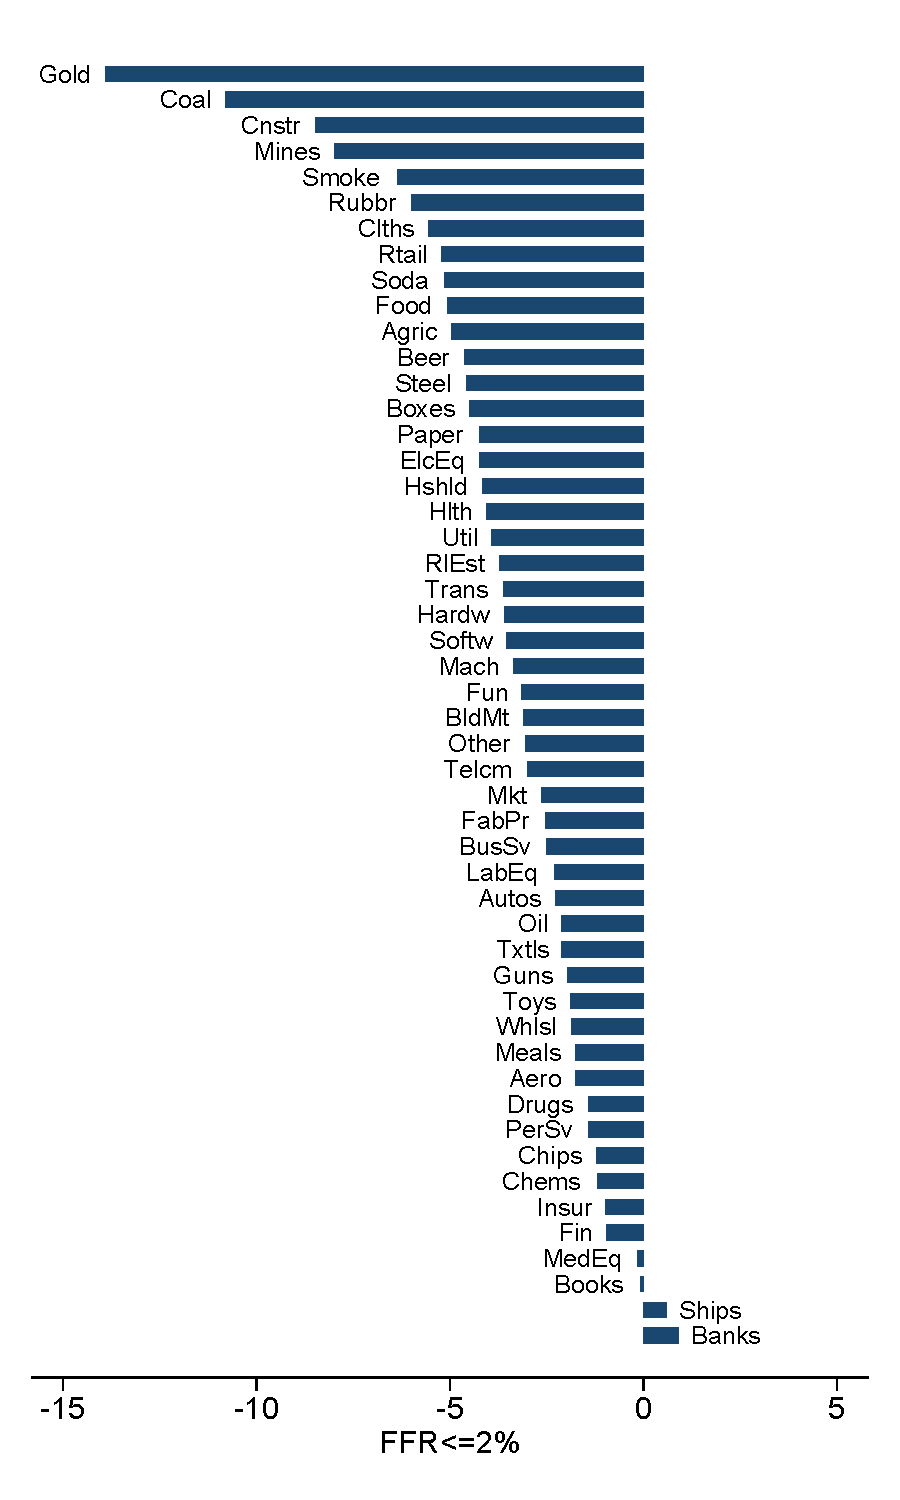
\includegraphics[scale=0.5]{../output/Figures/industry_fomc_bar_lt2}\caption{Monetary Policy Shocks and Bank Equity Returns\label{Fig: ind_stock_return}}
	\end{centering}
	{\footnotesize{The figure shows the sensitivity of bank and other industry stock portfolios to monetary policy shocks on the FOMC days. The bars present the coefficients from regressions of Fama-French 49 industry returns on the change in the two-year Treasury rate over a two-day window around FOMC meetings,  as in \cite{HansonStein2015}. The sample includes all scheduled FOMC meetings from 1994 to 2017. The left panel uses a sample in which the federal funds rate (FFR) is above 2\%. The right panel uses a sample in which the federal funds rate  is below or equal to 2\%. The industry returns are from Kenneth French's website. The two-year Treasury rate is obtained from the FRED database.}}
\end{figure}

\clearpage\newpage
\begin{table}[h]
		\caption{Summary Statistics 	\label{tab:sum_stats}}
		\vspace{5mm}
		
		%\footnotesize{\noindent In this table, we report summary statistics for our sample. The sample period is 1994--2017. The total size of the deposit market is defined as the sum of deposits, cash, and Treasury bills held by all U.S.\  households and non-financial corporations. The total size of the loan market is defined as the sum of U.S.\ corporate and household debt. Deposit and loan rates are calculated using interest expense and income. Expense related to fixed assets and salaries are scaled by total assets. Deposit shares, loan shares, deposit rates, loan rates, expenses related to fixed assets, salaries, and net noninterest expenses are reported in percentages. Asset maturity is reported in years. ``(vw)'' indicates an asset-weighted mean, and ``(ew)'' indicates an equal-weighted mean .  The data sources are the  Call Reports and the FDIC Summary of Deposits. \\}
		
		{
\def\sym#1{\ifmmode^{#1}\else\(^{#1}\)\fi}
\begin{tabular*}{\hsize}{@{\hskip\tabcolsep\extracolsep\fill}l*{1}{ccccccc}}
\toprule
                    &\multicolumn{7}{c}{}                                                                      \\
                    &        mean&          sd&         p10&         p25&         p50&         p75&         p90\\
\midrule
Deposit shares      &       0.079&       0.524&       0.003&       0.005&       0.009&       0.021&       0.077\\
\addlinespace
Loan shares         &       0.033&       0.207&       0.001&       0.002&       0.004&       0.009&       0.034\\
\addlinespace
Deposit rates       &       2.032&       1.292&       0.166&       0.873&       2.085&       3.150&       3.714\\
\addlinespace
Loan rates          &       6.921&       1.725&       4.540&       5.599&       6.959&       8.286&       9.061\\
\addlinespace
No. of branches     &      69.753&     315.678&       7.000&      11.000&      17.000&      34.000&      94.000\\
\addlinespace
No. of employees per branch&      18.338&      17.433&       9.109&      11.188&      14.306&      19.556&      28.500\\
\addlinespace
Expenses of fixed assets&       0.480&       0.165&       0.270&       0.347&       0.448&       0.584&       0.798\\
\addlinespace
Salaries            &       1.725&       0.486&       1.061&       1.348&       1.650&       2.036&       2.646\\
\addlinespace
Net noninterest expenses&       2.778&       0.830&       1.904&       2.246&       2.653&       3.142&       3.743\\
\addlinespace
Loan-to-deposit ratio&       0.815&       0.170&       0.598&       0.710&       0.821&       0.925&       1.022\\
\addlinespace
Borrowing-to-deposit ratio&       0.136&       0.138&       0.013&       0.041&       0.096&       0.181&       0.308\\
\addlinespace
Deposit-to-asset ratio&       0.805&       0.082&       0.691&       0.763&       0.822&       0.866&       0.895\\
\addlinespace
Book leverage       &      11.114&       2.577&       7.947&       9.408&      10.990&      12.656&      14.390\\
\addlinespace
Asset maturity      &       3.772&       1.402&       2.163&       2.764&       3.560&       4.604&       5.698\\
\bottomrule
\end{tabular*}
}

\end{table}



\begin{table}[h]
	\caption{Demand Estimation\label{tab:Demand}}
	\vspace{5mm}
	
	\footnotesize{In this table, we report the estimated deposit and loan demand parameters. The first column corresponds to the deposit demand parameter estimates. The second column contains the loan demand parameter estimates. Yield sensitivity ($\alpha$) refers to the average sensitivity of depositors (borrowers) to deposit rates (loan rates). Log No. of Branches ($\beta_1$) refers to the sensitivity of depositors (borrowers) to the log number of branches that each bank operates. Log No. of Employees ($\beta_1$) refers to the sensitivity of depositors (borrowers) to the log number of employees per branch. Yield sensitivity ($\sigma_\alpha$) refers to the dispersion in the sensitivity of depositors to deposit rates, with the dispersion  set at 0 for firms. The sample includes all U.S. commercial banks from 1994 to 2017. The data sources are the Call Reports and the FDIC Summary of Deposits.\\}
	
	\def\sym#1{\ifmmode^{#1}\else\(^{#1}\)\fi}\begin{tabular*}{\hsize}{@{\hskip\tabcolsep\extracolsep\fill}l*{2}{c}}\hline \hline &Deposit &Loan  \\ [1ex] \hline  Yield Sensitivity ($\alpha$)&0.967***&-1.462***\\
&[0.140]&[0.332]\\
\\
Log No. of Branches ($\beta_1$)&0.804***&0.948***\\
&[0.012]&[0.000]\\
\\
Log No. of Employees ($\beta_2$)&0.714***&0.631***\\
&[0.015]&[0.028]\\
\\
Yield Sensitivity Dispersion ($\sigma_{\alpha}$)&0.553***&\\
&[0.116]&\\
\\
\hline Sector F.E.&Y&Y \\ 
Time F.E.&Y&Y \\ 
Observations& 18062 &  18062\\
Adj. Rsq& 0.966 & 0.550\\
\hline \hline \end{tabular*}

\end{table}


\clearpage\newpage
	\begin{table}[h]
		\caption{Demand Estimation: Local Deposit Market\label{tab:Demand_Local}}
		\vspace{5mm}
		{
\def\sym#1{\ifmmode^{#1}\else\(^{#1}\)\fi}
\begin{tabular*}{\hsize}{@{\hskip\tabcolsep\extracolsep\fill}l*{1}{c}}
\hline\hline
                    &\multicolumn{1}{c}{(1)}\\
                    &\multicolumn{1}{c}{Deposit}\\
\hline
Yield sensitivity   &       0.903\sym{***}\\
                    &     [0.199]         \\
[1em]
Log number of branches&       0.509\sym{***}\\
                    &     [0.048]         \\
[1em]
Log number of employees&       0.322\sym{***}\\
                    &     [0.021]         \\
\hline
Bank F.E.           &         Yes         \\
Year-Sector F.E.    &         Yes         \\
Year-County F.E.    &         Yes         \\
Observations        &     377,309         \\
Adj. R-squared      &       0.399         \\
\hline\hline
\end{tabular*}
}

		\vspace{5mm}
		
		\small{This table reports the estimated deposit demand parameters using county-level market shares. Yield sensitivity refers to the average sensitivity of the depositors to deposit rates. Log number of branches refers to the sensitivity of the depositors to the log number of each bank's branches. Log number of employees refers the sensitivity of the depositors to the log number of employees per branch. The sample includes all U.S.\ commercial banks from 1994 to 2017. The data is from the Call Reports and the Summary of Deposits.}
	\end{table}

 \begin{table}[h]
 	\caption{Yield Sensitivity in the Deposit Market: Robustness \label{tab:demand_estimation_wage_deposit_1997_2017}}
 	\vspace{5mm}
 	{
\def\sym#1{\ifmmode^{#1}\else\(^{#1}\)\fi}
\begin{tabular*}{\hsize}{@{\hskip\tabcolsep\extracolsep\fill}l*{3}{c}}
\hline\hline
                    &\multicolumn{1}{c}{(1)}&\multicolumn{1}{c}{(2)}&\multicolumn{1}{c}{(3)}\\
                    &\multicolumn{1}{c}{Local wage}&\multicolumn{1}{c}{Bank expenses}&\multicolumn{1}{c}{All}\\
\hline
Yield sensitivity   &       0.668\sym{**} &       0.687\sym{***}&       0.687\sym{***}\\
                    &     (0.282)         &     (0.028)         &     (0.028)         \\
[1em]
Log number of branches&       0.769\sym{***}&       0.769\sym{***}&       0.769\sym{***}\\
                    &     (0.008)         &     (0.008)         &     (0.008)         \\
[1em]
Log number of employees&       0.674\sym{***}&       0.674\sym{***}&       0.674\sym{***}\\
                    &     (0.013)         &     (0.013)         &     (0.013)         \\
\hline
Bank F.E.           &         Yes         &         Yes         &         Yes         \\
Year-Sector F.E.    &         Yes         &         Yes         &         Yes         \\
Observations        &      11,394         &      11,394         &      11,394         \\
Adj. $ R^2$         &       0.970         &       0.969         &       0.969         \\
\hline\hline
\end{tabular*}
}

 	\vspace{5mm}
 	
 	\small{This table reports the estimated deposit demand parameters using alternative instruments. Column (1) uses local bank-teller wage data from the Bureau of Labor Statistics as an instrument, following \cite{Dick2008}. The instrument is   the weighted average of the local bank teller wages over the markets in which the bank operates, where the weight is the bank's deposit share in each market relative to its total deposits. Column (2) uses bank salary expenses and bank fixed assets expenses as instruments. Column (3) uses all  three instruments at the same time.  The sample period is from 1997 to 2017. The data are from the Call Reports, the Summary of Deposits, and the Bureau of Labor Statistics.}
 \end{table}
 
 
 
 
 \newpage
 \begin{table}[h]
 	\caption{Yield Sensitivity in the Loan Market: Robustness \label{tab:demand_estimation_wage_loan_1997_2017}}
 	\vspace{5mm}
 	{
\def\sym#1{\ifmmode^{#1}\else\(^{#1}\)\fi}
\begin{tabular*}{\hsize}{@{\hskip\tabcolsep\extracolsep\fill}l*{3}{c}}
\hline\hline
                    &\multicolumn{1}{c}{(1)}&\multicolumn{1}{c}{(2)}&\multicolumn{1}{c}{(3)}\\
                    &\multicolumn{1}{c}{Local wage}&\multicolumn{1}{c}{Bank expenses}&\multicolumn{1}{c}{All}\\
\hline
Yield sensitivity   &      -0.950         &      -1.149\sym{***}&      -1.134\sym{***}\\
                    &     (2.208)         &     (0.311)         &     (0.304)         \\
[1em]
Log number of branches&       0.913\sym{***}&       0.935\sym{***}&       0.933\sym{***}\\
                    &     (0.234)         &     (0.039)         &     (0.038)         \\
[1em]
Log number of employees&       0.652\sym{***}&       0.637\sym{***}&       0.638\sym{***}\\
                    &     (0.175)         &     (0.045)         &     (0.044)         \\
\hline
Bank F.E.           &         Yes         &         Yes         &         Yes         \\
Year-Sector F.E.    &         Yes         &         Yes         &         Yes         \\
Observations        &      11,394         &      11,394         &      11,394         \\
Adj. R-squared      &       0.840         &       0.772         &       0.777         \\
\hline\hline
\end{tabular*}
}

 	\vspace{5mm}
 	
 	\small{This table reports the estimated loan demand parameters using alternative instruments. Column (1) uses local wage data from the Bureau of Labor Statistics as an instrument, following \cite{Dick2008}. The instrument is   the weighted average of the local bank teller wages over the markets in which the bank operates, where the weight is the bank's deposit share in each market relative to its total deposits. Column (2) uses bank salary expenses and bank fixed assets expenses as instruments. Column (3) uses all  three instruments at the same time.  The sample period is from 1997 to 2017. The data are from the Call Reports, the Summary of Deposits, and the Bureau of Labor Statistics.}
 \end{table}
 


 

\clearpage
\newpage
\begin{table} 
	\caption{Monetary Policy Shocks and Bank Equity Returns on FOMC Days  \label{tab:stock_return_on_FOMC_days_r1}}
	\vspace{5mm}
	\footnotesize{\noindent In this table, we report the estimates of the relation  between bank equity returns and monetary policy shocks  on FOMC Days. Monetary policy shocks are measured by one-day changes in the two-year Treasury yield on FOMC days. HHI is the Herfindahl-Hirschman Index for the local deposit market in which a bank operates. Low is a dummy variable that equals one when the the starting level of the federal funds rate (FFR) is below 2\%. The control variables include market returns and term spreads. The sample includes all publicly traded U.S.\ banks from 1994 to 2017. The sample for columns (1) and (4) constitutes observations in which the starting level of the federal funds rate (FFR) is above 2\%. The sample for columns (2) and (5) constitutes observations in which the starting level of the federal funds rate is below 2\%.  The sample for columns (3) and (6) constitutes all observations.  We exclude observations during the collapse of the dot-com bubble (2000--2001) and the subprime financial crisis (2007-2009). Standard errors are clustered by time. \\}
	
	{
\def\sym#1{\ifmmode^{#1}\else\(^{#1}\)\fi}
\begin{tabular*}{\hsize}{@{\hskip\tabcolsep\extracolsep\fill}l*{6}{c}}
\hline\hline
                    &\multicolumn{1}{c}{(1)}&\multicolumn{1}{c}{(2)}&\multicolumn{1}{c}{(3)}&\multicolumn{1}{c}{(4)}&\multicolumn{1}{c}{(5)}&\multicolumn{1}{c}{(6)}\\
                    &\multicolumn{1}{c}{High}&\multicolumn{1}{c}{Low}&\multicolumn{1}{c}{All}&\multicolumn{1}{c}{High}&\multicolumn{1}{c}{Low}&\multicolumn{1}{c}{All}\\
\hline
Policy shock        &      -1.292\sym{**} &       2.202\sym{**} &      -1.292\sym{**} &      -0.639         &      -1.393         &      -0.639         \\
                    &     (0.615)         &     (0.879)         &     (0.612)         &     (0.653)         &     (0.852)         &     (0.649)         \\
[1em]
Low*Policy shock    &                     &                     &       3.494\sym{***}&                     &                     &      -0.754         \\
                    &                     &                     &     (1.069)         &                     &                     &     (1.069)         \\
[1em]
HHI*Policy shock    &                     &                     &                     &      -0.134         &       0.562\sym{***}&      -0.134         \\
                    &                     &                     &                     &     (0.145)         &     (0.153)         &     (0.144)         \\
[1em]
Low*HHI*Policy shock&                     &                     &                     &                     &                     &       0.696\sym{***}\\
                    &                     &                     &                     &                     &                     &     (0.210)         \\
\hline
Control             &         Yes         &         Yes         &         Yes         &         Yes         &         Yes         &         Yes         \\
Observations        &      27,257         &      33,805         &      61,062         &      27,257         &      33,805         &      61,062         \\
Adj. $ R^2$         &       0.015         &       0.123         &       0.074         &       0.016         &       0.125         &       0.075         \\
\hline\hline
\end{tabular*}
}

\end{table}


\clearpage
\begin{table}[h]
	\caption{Monetary Policy Shocks and Bank Equity Returns on FOMC Days \label{tab:stock_return_on_FOMC_days_Appendix}}
	\vspace{5mm}
	{
\def\sym#1{\ifmmode^{#1}\else\(^{#1}\)\fi}
\begin{tabular*}{\hsize}{@{\hskip\tabcolsep\extracolsep\fill}l*{4}{c}}
\hline\hline
                    &\multicolumn{1}{c}{(1)}&\multicolumn{1}{c}{(2)}&\multicolumn{1}{c}{(3)}&\multicolumn{1}{c}{(4)}\\
                    &\multicolumn{1}{c}{High FFR}&\multicolumn{1}{c}{Low FFR}&\multicolumn{1}{c}{High FFR}&\multicolumn{1}{c}{Low FFR}\\
\hline
Policy shock        &      -1.365\sym{**} &       1.290         &      -0.103         &      -2.623         \\
                    &     [0.597]         &     [1.326]         &     [1.019]         &     [2.108]         \\
[1em]
HHI*Policy shock    &                     &                     &      -0.303         &       0.740\sym{**} \\
                    &                     &                     &     [0.262]         &     [0.372]         \\
[1em]
$\Delta$ Term spread&      -0.605         &       2.944\sym{***}&      -0.471         &       2.644\sym{**} \\
                    &     [0.688]         &     [1.103]         &     [0.696]         &     [1.070]         \\
[1em]
Market return       &       0.298\sym{***}&       0.727\sym{***}&       0.296\sym{***}&       0.730\sym{***}\\
                    &     [0.074]         &     [0.069]         &     [0.073]         &     [0.069]         \\
\hline
Observations        &      27,257         &      33,805         &      27,257         &      33,805         \\
Adj, R-squared      &       0.015         &       0.124         &       0.016         &       0.125         \\
\hline\hline
\end{tabular*}
}

	\vspace{5mm}
	
	\footnotesize{\noindent This table reports the estimates of the relation between bank equity returns and monetary policy shocks  on FOMC days. Monetary policy shocks are measured by the one-day changes in the one-year Treasury yield on FOMC days. HHI is the Herfindahl-Hirschman Index of the local deposit market in which the bank operates.  The sample for columns (1) and (3) constitutes observations in which the starting level of the federal funds rate is above 2\%. The sample for columns (2) and (4) constitutes observations in which the starting level of the federal funds rate is below 2\%.   We exclude observations during the collapse of the dot-com bubble (2000-2001) and the  financial crisis (2007-2009). The standard errors are clustered by time.}
	\label{tab:stock_return_on_FOMC_days_one_year}
\end{table}


\clearpage\newpage
\begin{table} 
	\caption{Effects of Low Rates on Banks with Different Deposit Market Power  \label{tab:reversal_lending}}
	\vspace{5mm}
	\footnotesize{\noindent We report the estimates of the effect of low interest rates on banks with different deposit market power. HHI is the average Herfindahl-Hirschman Index of the local deposit markets in which a bank operates. Low is a dummy variable that equals one when the federal funds rate is below 2\%. Each column is identified by the dependent variable. The control variables include lagged assets, lending, deposits, equity, deposit rate, loan rate, bank fixed effects, and time fixed effects. The sample includes all U.S.\ banks from 2000Q1 to 2004Q1. Standard errors are clustered by time. \\}
	{
\def\sym#1{\ifmmode^{#1}\else\(^{#1}\)\fi}
\begin{tabular*}{\hsize}{@{\hskip\tabcolsep\extracolsep\fill}l*{4}{c}}
\hline\hline
                    &\multicolumn{1}{c}{(1)}&\multicolumn{1}{c}{(2)}&\multicolumn{1}{c}{(3)}&\multicolumn{1}{c}{(4)}\\
                    &\multicolumn{1}{c}{Equity}&\multicolumn{1}{c}{Equity}&\multicolumn{1}{c}{Loan}&\multicolumn{1}{c}{Loan}\\
\hline
HHI*Low             &      -0.232\sym{***}&      -0.083\sym{***}&      -0.252\sym{***}&      -0.055\sym{***}\\
                    &     (0.007)         &     (0.006)         &     (0.008)         &     (0.006)         \\
\hline
Control             &          No         &         Yes         &          No         &         Yes         \\
Bank F.E.           &         Yes         &         Yes         &         Yes         &         Yes         \\
Time F.E.           &         Yes         &         Yes         &         Yes         &         Yes         \\
Observations        &     129,950         &     127,912         &     129,339         &     127,885         \\
Adj. \(R^{2}\)      &       0.984         &       0.990         &       0.981         &       0.990         \\
\hline\hline
\end{tabular*}
}

\end{table}


\clearpage\newpage
\begin{table}[h]
	\caption{Data Moments: Full Sample}
	\vspace{5mm}
	\begin{tabular*}{\hsize}{@{\hskip\tabcolsep\extracolsep\fill}l*{2}{c}}\hline \hline & {Actual Moment}  &    \\ [1ex] \hline  Dividend yield&0.034&\\
MB&2.060&\\
Leverage&11.197&\\
Borrowing/Deposits&0.299&\\
Borrowing/Deposits (sd)&0.204&\\
Borrowing/Deposits (demeaned sd)&0.126&\\
Deposits to Assets Ratio&0.699&\\
Net noninterest expenses&0.012&\\
Deposit Spreads&1.297&\\
Loan Spreads&2.032&\\
Deposit Spreads - FFR Sensitivity&0.441&\\
Loan Spreads - FFR Sensitivity&-0.125&\\
Total Credit - FFR Sensitivity&-0.995&\\
Total Credit - FFR Sensitivity (se)&0.299&\\
Bank Loan - FFR Sensitivity&-1.592&\\
Bank Loan - FFR Sensitivity (se)&0.503&\\
Repricing Duration&3.429&\\
Repricing Duration (sd)&1.445&\\
Reserve Ratio&2.495&\\
Depositor Sensitivity to Deposit Rates&0.967&\\
Depositor Sensitivity to Deposit Rates (se)&0.140&\\
Dispersion of Depositor Sensitivity to Deposit Rates&0.553&\\
Dispersion of Depositor Sensitivity to Deposit Rates (se)&0.116&\\
Borrower Sensitivity to Loan Rates&-1.462&\\
Borrower Sensitivity to Loan Rates (se)&0.332&\\
Convenience of Holding Cash ($q_c$)&1.986&\\
Convenience of Holding Cash (se)&0.242&\\
Convenience of Holding Deposits ($q_d$)&3.441&\\
Convenience of Holding Deposits (se)&0.251&\\
Convenience of Borrowing Loans ($q_l$)&1.152&\\
Convenience of Borrowing Loans (se)&1.232&\\
Number of Banks&5.592&\\
\hline \hline \end{tabular*}

	\vspace{5mm}
\end{table}


\clearpage\newpage
\begin{table}[h]
	\caption{Data Moments: Early Sample}
	\vspace{5mm}
	\begin{tabular*}{\hsize}{@{\hskip\tabcolsep\extracolsep\fill}l*{2}{c}}\hline \hline & {Actual Moment}  &    \\ [1ex] \hline  Dividend yield&0.031&\\
MB&2.767&\\
Leverage&12.460&\\
Borrowing/Deposits&0.342&\\
Borrowing/Deposits (sd)&0.220&\\
Borrowing/Deposits (demeaned sd)&0.103&\\
Deposits to Assets Ratio&0.679&\\
Net noninterest expenses&0.013&\\
Deposit Spreads&1.951&\\
Loan Spreads&1.827&\\
Deposit Spreads - FFR Sensitivity&0.488&\\
Loan Spreads - FFR Sensitivity&0.018&\\
Total Credit - FFR Sensitivity&-0.995&\\
Total Credit - FFR Sensitivity (se)&0.299&\\
Bank Loan - FFR Sensitivity&-1.592&\\
Bank Loan - FFR Sensitivity (se)&0.503&\\
Repricing Duration&3.178&\\
Repricing Duration (sd)&1.402&\\
Reserve Ratio&2.767&\\
Depositor Sensitivity to Deposit Rates&0.743&\\
Depositor Sensitivity to Deposit Rates (se)&0.165&\\
Dispersion of Depositor Sensitivity to Deposit Rates&0.423&\\
Dispersion of Depositor Sensitivity to Deposit Rates (se)&0.144&\\
Borrower Sensitivity to Loan Rates&-1.017&\\
Borrower Sensitivity to Loan Rates (se)&0.054&\\
Convenience of Holding Cash ($q_c$)&2.761&\\
Convenience of Holding Cash (se)&0.387&\\
Convenience of Holding Deposits ($q_d$)&3.463&\\
Convenience of Holding Deposits (se)&0.357&\\
Convenience of Borrowing Loans ($q_l$)&-0.015&\\
Convenience of Borrowing Loans (se)&0.087&\\
Number of Banks&7.056&\\
\hline \hline \end{tabular*}

	\vspace{5mm}
\end{table}


\clearpage\newpage
\begin{table}[h]
	\caption{Data Moments: Late Sample}
	\vspace{5mm}
	\begin{tabular*}{\hsize}{@{\hskip\tabcolsep\extracolsep\fill}l*{2}{c}}\hline \hline & {Actual Moment}  &    \\ [1ex] \hline  Dividend yield&0.036&\\
MB&1.538&\\
Leverage&9.933&\\
Borrowing/Deposits&0.256&\\
Borrowing/Deposits (sd)&0.173&\\
Borrowing/Deposits (demeaned sd)&0.106&\\
Deposits to Assets Ratio&0.719&\\
Net noninterest expenses&0.012&\\
Deposit Spreads&0.643&\\
Loan Spreads&2.238&\\
Deposit Spreads - FFR Sensitivity&0.489&\\
Loan Spreads - FFR Sensitivity&-0.139&\\
Total Credit - FFR Sensitivity&-0.995&\\
Total Credit - FFR Sensitivity (se)&0.299&\\
Bank Loan - FFR Sensitivity&-1.592&\\
Bank Loan - FFR Sensitivity (se)&0.503&\\
Repricing Duration&3.590&\\
Repricing Duration (sd)&1.448&\\
Reserve Ratio&2.224&\\
Depositor Sensitivity to Deposit Rates&0.924&\\
Depositor Sensitivity to Deposit Rates (se)&0.400&\\
Dispersion of Depositor Sensitivity to Deposit Rates&0.528&\\
Dispersion of Depositor Sensitivity to Deposit Rates (se)&0.279&\\
Borrower Sensitivity to Loan Rates&-1.454&\\
Borrower Sensitivity to Loan Rates (se)&0.079&\\
Convenience of Holding Cash ($q_c$)&-0.444&\\
Convenience of Holding Cash (se)&0.430&\\
Convenience of Holding Deposits ($q_d$)&2.336&\\
Convenience of Holding Deposits (se)&0.470&\\
Convenience of Borrowing Loans ($q_l$)&1.804&\\
Convenience of Borrowing Loans (se)&0.201&\\
Number of Banks&5.105&\\
\hline \hline \end{tabular*}

	\vspace{5mm}
\end{table}


\clearpage\newpage
\begin{table}[h]
	\caption{Data Moments: Big Banks }
	\vspace{5mm}
	\begin{tabular*}{\hsize}{@{\hskip\tabcolsep\extracolsep\fill}l*{2}{c}}\hline \hline & {Actual Moment}  &    \\ [1ex] \hline  Dividend yield&0.036&\\
Leverage&11.359&\\
Borrowing/Deposits&0.355&\\
Borrowing/Deposits (sd)&0.190&\\
Borrowing/Deposits (demeaned sd)&0.133&\\
Deposits to Assets Ratio&0.666&\\
Net noninterest expenses&0.010&\\
Deposit Spreads&1.317&\\
Loan Spreads&1.770&\\
Deposit Spreads - FFR Sensitivity&0.415&\\
Loan Spreads - FFR Sensitivity&-0.143&\\
Total Credit - FFR Sensitivity&-0.995&\\
Total Credit - FFR Sensitivity (se)&0.299&\\
Bank Loan - FFR Sensitivity&-1.592&\\
Bank Loan - FFR Sensitivity (se)&0.503&\\
Repricing Duration&3.341&\\
Repricing Duration (sd)&1.337&\\
Reserve Ratio&2.466&\\
Depositor Sensitivity to Deposit Rates&1.127&\\
Depositor Sensitivity to Deposit Rates (se)&0.276&\\
Dispersion of Depositor Sensitivity to Deposit Rates&0.645&\\
Dispersion of Depositor Sensitivity to Deposit Rates (se)&0.199&\\
Borrower Sensitivity to Loan Rates&-1.679&\\
Borrower Sensitivity to Loan Rates (se)&0.103&\\
Convenience of Holding Cash ($q_c$)&1.986&\\
Convenience of Holding Cash (se)&0.242&\\
Convenience of Holding Deposits ($q_d$)&3.441&\\
Convenience of Holding Deposits (se)&0.251&\\
Convenience of Borrowing Loans ($q_l$)&1.152&\\
Convenience of Borrowing Loans (se)&1.232&\\
Number of Banks&5.592&\\
\hline \hline \end{tabular*}

	\vspace{5mm}
\end{table}


\clearpage\newpage
\begin{table}[h]
	\caption{Data Moments: Small Banks}
	\vspace{5mm}
	\begin{tabular*}{\hsize}{@{\hskip\tabcolsep\extracolsep\fill}l*{2}{c}}\hline \hline & {Actual Moment}  &    \\ [1ex] \hline  Dividend yield&0.036&\\
Leverage&10.776&\\
Borrowing/Deposits&0.153&\\
Borrowing/Deposits (sd)&0.172&\\
Borrowing/Deposits (demeaned sd)&0.087&\\
Deposits to Assets Ratio&0.784&\\
Net noninterest expenses&0.019&\\
Deposit Spreads&1.245&\\
Loan Spreads&2.716&\\
Deposit Spreads - FFR Sensitivity&0.501&\\
Loan Spreads - FFR Sensitivity&-0.113&\\
Total Credit - FFR Sensitivity&-0.995&\\
Total Credit - FFR Sensitivity (se)&0.299&\\
Bank Loan - FFR Sensitivity&-1.592&\\
Bank Loan - FFR Sensitivity (se)&0.503&\\
Repricing Duration&3.685&\\
Repricing Duration (sd)&1.697&\\
Reserve Ratio&2.570&\\
Depositor Sensitivity to Deposit Rates&1.153&\\
Depositor Sensitivity to Deposit Rates (se)&0.094&\\
Dispersion of Depositor Sensitivity to Deposit Rates&0.660&\\
Dispersion of Depositor Sensitivity to Deposit Rates (se)&0.226&\\
Borrower Sensitivity to Loan Rates&-0.628&\\
Borrower Sensitivity to Loan Rates (se)&0.041&\\
Convenience of Holding Cash ($q_c$)&1.986&\\
Convenience of Holding Cash (se)&0.242&\\
Convenience of Holding Deposits ($q_d$)&3.441&\\
Convenience of Holding Deposits (se)&0.251&\\
Convenience of Borrowing Loans ($q_l$)&1.152&\\
Convenience of Borrowing Loans (se)&1.232&\\
Number of Banks&5.592&\\
\hline \hline \end{tabular*}

	\vspace{5mm}
\end{table}



\clearpage \newpage {\color{black}
	\singlespacing
	\bibliographystyle{jf}
	
	\bibliography{appendix}
	
}
\end{document}